\documentclass[french]{beamer}

\mode<presentation> {
  \usetheme{Warsaw}
}

\usepackage[english]{babel}
\usepackage[utf8]{inputenc}
\usepackage{times}
\usepackage[T1]{fontenc}
\usepackage{hyperref}
\usepackage{yhmath} %pour la commande \widering (intérieur topologique)
\usepackage{algorithm2e}

\DeclareMathOperator*{\argmin}{argmin}
\DeclareMathOperator*{\argmax}{argmax}
\DeclareMathOperator*{\sup2}{sup}
\DeclareMathOperator*{\inf2}{inf}
\DeclareMathOperator*{\max2}{max}
\DeclareMathOperator*{\min2}{min}


\newcommand{\Max}{\mathop{\mathrm{Max}}}
\newcommand{\R}{\mathbb{R}}
\newcommand{\Z}{\mathbb{Z}}
\newcommand{\E}{\mathbb{E}}
\newcommand{\xx}{\mathbf{x}}
\newcommand{\yy}{\mathbf{y}}
\newcommand{\zz}{\mathbf{z}}
\newcommand{\bxi}{\boldsymbol{\xi}}
\newcommand{\nyq}{\boldsymbol{\eta}}
\newcommand{\tv}{\mathrm{TV}}
\newcommand{\si}{\mathrm{SI}}
\newcommand{\m}{\mathrm{m}}
\newcommand{\num}{\mathrm{num}}
\newcommand{\denom}{\mathrm{denom}}
\renewcommand{\v}{\mathrm{v}}
\newcommand{\gpc}{\mathrm{GPC}}
\renewcommand{\P}{\mathbb{P}}
\newcommand{\var}{\mathbb{V}\mathrm{ar}}
\newcommand{\sgn}{\mathrm{sgn}}
\renewcommand{\widering}[1]{\ring{\wideparen{#1}}}

\newcommand{\I}{\textbf{I}}
\newcommand{\B}{\textbf{B}}
\newcommand{\N}{\textbf{N}}
\newcommand{\Nd}{\textbf{N$_d$}}
\newcommand{\kernel}{\textbf{k}}
\newcommand{\ksize}{\textbf{k$_{size}$}}
\newcommand{\Isize}{\textbf{n}}

\theoremstyle{plain}
\newtheorem{theoreme}{Th\'eor\`eme}[section]
\newtheorem{algo}{Algorithme}[section]
\newtheorem{lemme}[theoreme]{Lemme}
\newtheorem{proposition}[theoreme]{Proposition}
\newtheorem{corollaire}[theoreme]{Corollaire}
\theoremstyle{remark}
\newtheorem{exemple}{Exemple}[section]

\hypersetup{
      pdfpagemode = FullScreen,% afficher le pdf en plein écran
      pdfauthor   = {Yohann Salaun },%
      pdftitle    = {Image Deblurring with Blurred/Noisy Image Pairs]},%
      pdfsubject  = {Présentation GTTJD},%
      pdfkeywords = {deblurring,denoising},%
      pdfcreator  = {PDFLaTeX},%
      pdfproducer = {PDFLaTeX}%
}

% Faire apparaître un sommaire avant chaque section
\AtBeginSection[]{
   \begin{frame}
   \begin{center}{\Large Plan }\end{center}
   %%% affiche en début de chaque section, les noms de sections et
   %%% noms de sous-sections de la section en cours.
   \tableofcontents[currentsection,hideothersubsections]
   \end{frame} 
}

\title[Image Deblurring with Blurred/Noisy Image Pairs]{Image Deblurring \\ with Blurred/Noisy Image Pairs}
\author{Yohann Salaun}



\author[Yohann Salaun] 
{Yohann Salaun}

\institute[MVA - Introduction à l'imagerie Numérique] 
{MVA - Introduction à l'imagerie Numérique}

\date[25 Janvier 2013] % (facultatif)
{-- Soutenance de Projet --\\ 25 Janvier 2013}

\addtobeamertemplate{footline}{\insertframenumber/\inserttotalframenumber} %numéroter des slides

\begin{document}

\begin{frame}
  \titlepage
\end{frame}

\begin{frame}{Table of contents}
  \tableofcontents
\end{frame}

%%%%%%%%%%%%%%%%%%%%%%%%%%% Fin de l'en-tete %%%%%%%%%%%%%%%%%%%%%%%%%%%%

\section{Introduction}

\begin{frame}{Image deblurring with blurred/noisy image pairs}

\begin{figure}[ht]
\begin{center}
	\begin{tabular}{c}	
		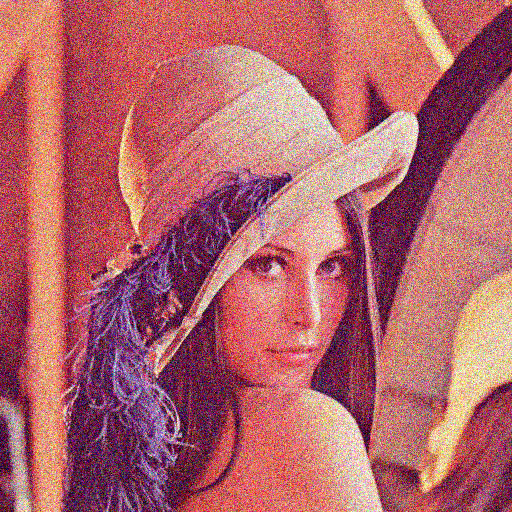
\includegraphics[scale=0.18]{images/lena_noisy.jpg}
		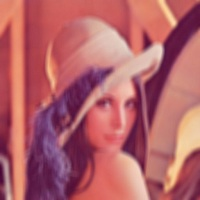
\includegraphics[scale=0.18]{images/lena_blurred.jpg}
		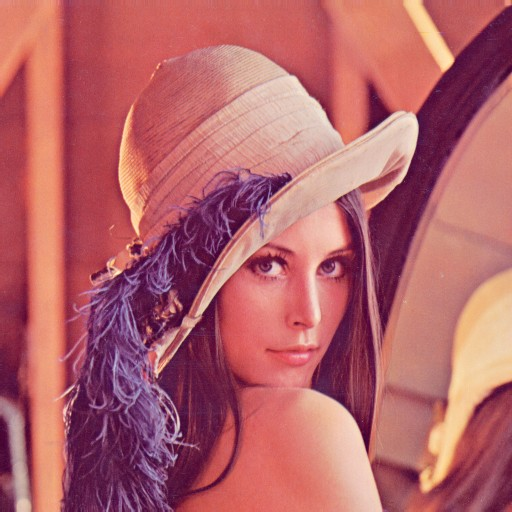
\includegraphics[scale=0.18]{images/lena.jpg}
	\end{tabular}
\end{center}
\end{figure}
\small
\emph{Image deblurring with blurred/noisy image pairs}, Lu Yuan, Jian Sun, Long Quan, and Heung-Yeung Shum, Siggraph'07, 2007

\end{frame}


\section{Algorithm Overview}

\begin{frame}{Algorithm Overview}

\textbf{Input} : Noisy picture \N, Blurry picture \B, estimated kernel size \ksize\\
\textbf{Output} : Estimated picture \I, estimated kernel \kernel \\
	\Nd = denoise(\N)\\ 
	\I  = \Nd  \\
	\While{ change $> \epsilon$}{
		\textbf{Estimate} kernel \kernel\ with \I\ and \B\ s.t. \B\ = \I\ $\otimes$ \kernel.\\
		\textbf{Deconvolute} blurred picture \B.\\
		\textbf{Mix} informations to improve estimation \I.\\
		\textbf{Compute} \textit{change} between 2 iterations.
	}
\end{frame}

\section{Theoretical Description}

\subsection{Initialization}

\begin{frame}{Initialization}

\begin{figure}[ht]
\begin{center}
	\begin{tabular}{c}	
		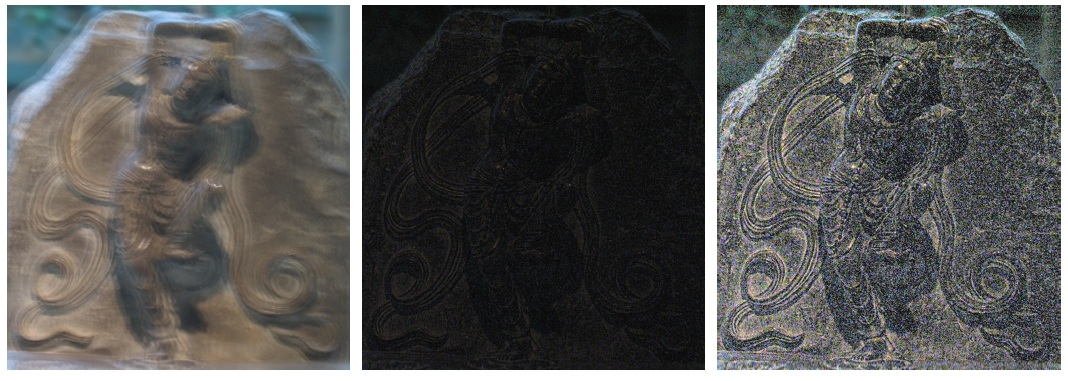
\includegraphics[scale=0.35]{images/enhanced.jpg}
	\end{tabular}
	\label{enhanced}
\end{center}
\end{figure}
\small

\emph{Image denoising using scale mixtures of gaussians in the wavelet domain}, J. Portilla, V. Strela, M. Wainwright, and E.P. Simoncelli, IEEE, Trans. on Image Processing 12, 11, 1338–1351, 2003.

\end{frame}

\subsection{Kernel Estimation}

\begin{frame}{Kernel Equations}

Kernel equation into vector-matrix form:
\[
	\B = \I\kernel
\]

\pause

Tikhonov regularization method:
\[
min_{\kernel \in \mathbb{R}^{\ksize}} ||\I\kernel - \B||_2^2 + \lambda^2||\kernel||_2^2, \ \ s.t. \ \ \kernel \in \mathbb{R}^{+\ksize} \ \ and \ \ ||\kernel||_1 = 1 
\]

\end{frame}

\begin{frame}{Gradient Descent}

\begin{itemize}
	\item[$\bullet$] $\kernel^0$ is initialized as the delta function.
	\pause
	\item[$\bullet$] $\kernel^{n+1} = \kernel^n + \tau\nabla F(\kernel^n) = \kernel^n + 2\tau(\I^T\B - (\I^T\I +\lambda^2Id)\kernel^n)$
	\pause
	\item[$\bullet$] $\kernel^{n+1} = Proj_K(\kernel^{n+1})$
\end{itemize}

\pause

with $Proj_K$ computed by :
\begin{itemize}
	\item[$\bullet$] turning positive the kernel coefficients $\kernel_i= max(\kernel_i, 0)$
	\pause
	\item[$\bullet$] normalizing the kernel $\kernel = \frac{\kernel}{||\kernel||}$
\end{itemize}

\end{frame}

\subsection{Deconvolution}

\begin{frame}{Richardson-Lucy Algorithm}

Iterative method for deconvolution :
\[
	\I^{k+1} _i= \I^k_i \sum_{j}\frac{\B_j}{(\kernel \otimes \I^k)_j} \kernel_j[i]
\]
where $\kernel_j[i]$ is the $j^{th}$ coefficients of the kernel \kernel\ centered in pixel $i$.

\end{frame}

\begin{frame}{Residual Deconvolution}

Residual instead of pictures to limit ringing artifacts :
\begin{itemize}
	\item[$\bullet$] $\Delta \I = \I - \Nd$
	\item[$\bullet$] $\Delta \B = \Delta \I \otimes \kernel = \B - \Nd \otimes \kernel$
\end{itemize}
\pause
Offset added to avoid zero values issues :
\[
	\Delta \I^{k+1}_i + 1= (\Delta\I^k_i+1) \sum_{j}\frac{\Delta\B_j + 1}{(\kernel \otimes \Delta\I^k)_j + 1} \kernel_j[i]
\]

\end{frame}

\subsection{De-ringing}	

\begin{frame}{Gain-controlled RL deconvolution}

\[
	\I^{k+1} _i= I_{GAIN}[i](\I^k_i \sum_{j}\frac{\B_j}{(\kernel \otimes \I^k)_j} \kernel_j[i])
\]
\pause
where $I_{GAIN}$ controls the increase of contrast :

\[
	I_{GAIN} \sim (1 - \alpha) + \alpha \| \nabla \Nd \|
\]
where $\alpha = 0.8$ in the article

\end{frame}

\begin{frame}{Final Deconvolution}

\begin{itemize}
	\item[$\bullet$] RL-deconvolution on $\I_{RL} = RL(\I)$
	\pause
	\item[$\bullet$] Gain-controlled RL-deconvolution on $\I_{g} = RL_{gain}(\I)$
	\pause
	\item[$\bullet$] Compute a detail layer $\I_d = \I_{RL} - F(\I_{RL})$ where $F$ is a low-pass filter such as the bilateral filter
	\pause
	\item[$\bullet$] Compose the detail layer $\I_d$ and the base layer $\I_g$
\end{itemize}

\end{frame}

\section{Results}

\begin{frame}{$5 \times 5$ kernel}

\begin{figure}
\begin{center}
	\begin{tabular}{c}	
		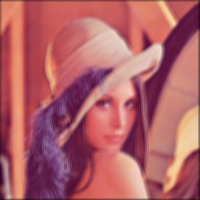
\includegraphics[scale=0.5]{images/blurred_5px.png}
		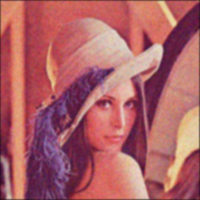
\includegraphics[scale=0.5]{images/denoised_5px.png}
		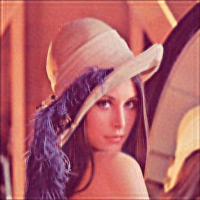
\includegraphics[scale=0.5]{images/estimation_5px.png}
		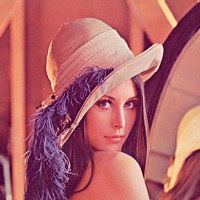
\includegraphics[scale=0.5]{images/original_5px.png}\\
		
\includegraphics[scale=0.5]{images/kernels_5px.png}
	\end{tabular}
\end{center}
\end{figure}

\end{frame}

\begin{frame}{$9 \times 9$ kernel}

\begin{figure}
\begin{center}
	\begin{tabular}{c}	
		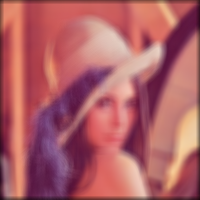
\includegraphics[scale=0.5]{images/blurred_9px.png}
		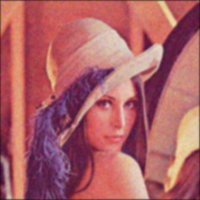
\includegraphics[scale=0.5]{images/denoised_9px.png}
		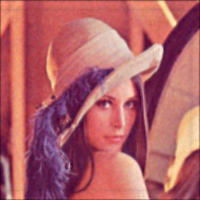
\includegraphics[scale=0.5]{images/estimation_9px.png}
		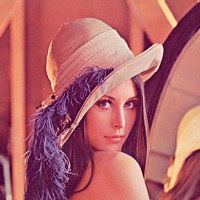
\includegraphics[scale=0.5]{images/original_5px.png}\\
		
\includegraphics[scale=0.5]{images/kernels_5px.png}
	\end{tabular}
\end{center}
\end{figure}

\end{frame}

\begin{frame}{Different initialization}

\begin{figure}
\begin{center}
	\begin{tabular}{c}	
		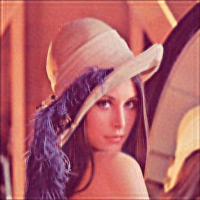
\includegraphics[scale=0.5]{images/estimation_5px.png}
		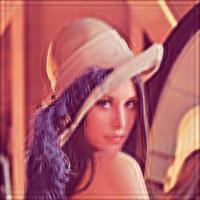
\includegraphics[scale=0.5]{images/estimation_0.png}
		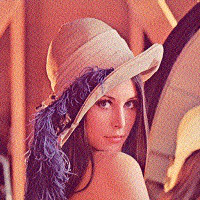
\includegraphics[scale=0.5]{images/estimation_N.png}\\
		
\includegraphics[scale=0.5]{images/kernels_5px.png}
		
\includegraphics[scale=0.5]{images/kernels_0.png}
		
\includegraphics[scale=0.5]{images/kernels_N.png}
	\end{tabular}
\end{center}
\end{figure}

\end{frame}

\begin{frame}{Kernel size}

\begin{figure}
\begin{center}
	\begin{tabular}{c}	
		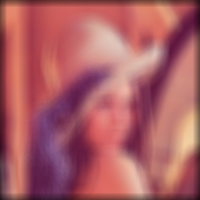
\includegraphics[scale=0.5]{images/blurred_15_5.png}
		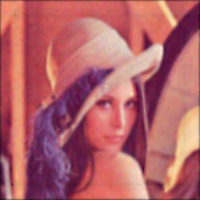
\includegraphics[scale=0.5]{images/estimation_15_5.png}
		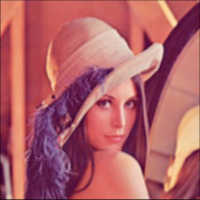
\includegraphics[scale=0.5]{images/blurred_3_9.png}
		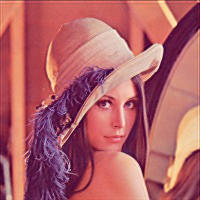
\includegraphics[scale=0.5]{images/estimation_3_9.png}
	\end{tabular}
\end{center}
\end{figure}

\end{frame}

\begin{frame}{Article results}

\begin{figure}
\begin{center}
	\begin{tabular}{c}	
		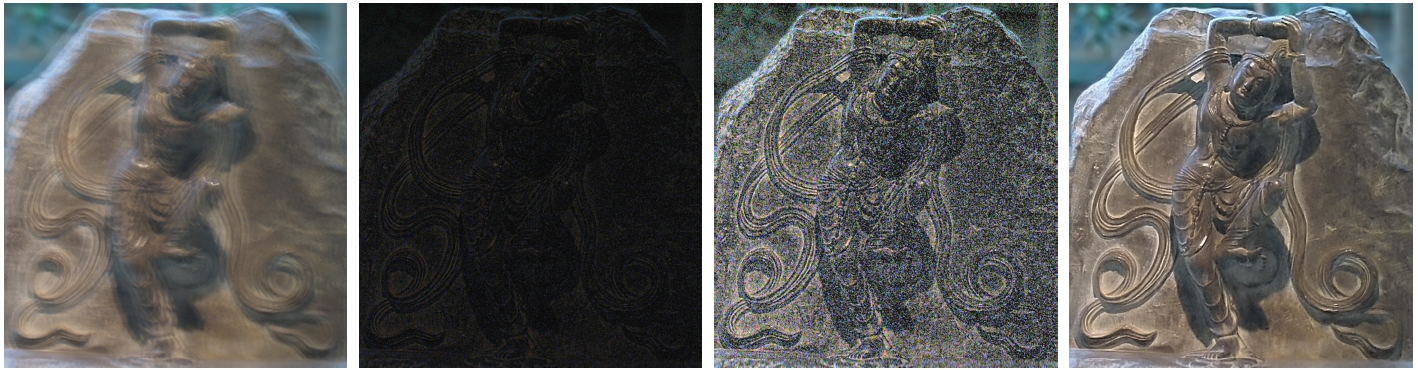
\includegraphics[scale=0.28]{images/results.png}
	\end{tabular}
\end{center}
\end{figure}

\end{frame}

\end{document}
